\chapter{Bayesovské testování hypotéz}
Testujeme hypotézy $\hypothesis{\t\in\Theta_0}{\t\in\Theta_1} (\Theta
=\Theta_0 \biguplus \Theta_1)$. Znáhodníme $\t\sim\pi(\t)$ apriorní informaci (vlastní/nevlastní/konstanta).
\begin{description}
	\item[apriorní test $H_0$] $\PP^\pi(H_0)=\PP^\pi(\t\in\Theta_0)\stackrel{?}{>}\frac{1}{2}$, potom $H_0$ přijmeme.
	\item[aposteriorní test $H_0$] máme $\pi(\t)$, z toho data $\textbf{X}\sim\fex$, z toho aktualizujeme $\pi(\t|\textbf{x})$. Nakonec tedy 
	\[
	\begin{split}
	 \PP^\pi(H_0|\textbf{x})=\PP^\pi(\t\in\Theta_0|\textbf{x})&\stackrel{?}{>}\frac{1}{2}\quad\Rightarrow\quad H_0\text{ přijmeme.}\\
	 \int_{\Theta_0}\pi(\t|\textbf{x})\d\t & \lessgtr \frac{1}{2},
	\end{split}
	\]
	kde $\pi(\t|\textbf{x})\to \frac{f\pi(\t)}{\int_\Theta f\pi(\t)\d\t}$.
\end{description}

Máme tedy $\mathscr{D}=\{0,~1\}=\{\text{no }H_0,~\text{yes }H_0\}$ a 
$$ \tau(\t)=I_{\Theta_0}=\begin{cases}
1& \t\in\Theta_0~(H_0\text{ platí}),\\0& \t\in\Theta_1~(H_1\text{ platí}),
\end{cases}$$ s čímž přišel Neyman s Pearsonem (a Fisherem) už kolem roku 1950.
\begin{theorem}
	Volme $$L_{a_0-a_1}(\t,\delta)=\begin{cases}
	0&\delta=I_{\Theta_0}(\t)=\tau(\t)~(\text{trefa}),\\a_0& \t\in\Theta_0(H_0)\wedge \delta=0~(\text{chyba I. druhu}),\\a_1& \t\in\Theta_1(H_1)\wedge \delta=1~(\text{chyba II. druhu}),
	\end{cases}$$
	kde $W\subset\R^n$, $\PP(\textbf{X}\in W|H_0)\leq \alpha$ a $\beta$ je síla testu. Pak $$\delta^\pi=\begin{cases}
	1& \text{pokud }\PP^\pi(\t\in\Theta_0|\textbf{x})>\frac{a_1}{a_0+a_1},\\
	0& \text{pokud }\PP^\pi(\t\in\Theta_0|\textbf{x})\leq\frac{a_1}{a_0+a_1},
	\end{cases}$$ kde $\frac{a_1}{a_0+a_1}=\frac{1}{1+\frac{a_0}{a_1}}$ je závislá na $\frac{a_0}{a_1}$. Pro $a_0=a_1=1$ je pak hranice $\frac{1}{2}$.
	\begin{proof}
		Máme
		\[
		\begin{split}
		\rho(\pi,\delta|\textbf{x})&=\E^\pi\big[L\big(\t,\delta(\textbf{x})\big)\big| \textbf{x}\big]=0\cdot\PP(...)+a_0\cdot \PP^\pi(\t\in\Theta_0|\textbf{x})I_{\{0\}}(\delta)+a_1 \PP^\pi (\t\in\Theta_0|\textbf{x})I_{\{1\}}(\delta)=\\&=\begin{cases}
		a_0 \PP^\pi(\t\in\Theta_0|\textbf{x})&\text{pokud }\delta(\textbf{x})=0,\\
		a_1 \PP^\pi(\t\in\Theta_1|\textbf{x})&\text{pokud }\delta(\textbf{x})=1,
		\end{cases}
		\end{split}
		\] 
		
		\begin{figure}[h]
			\centering
			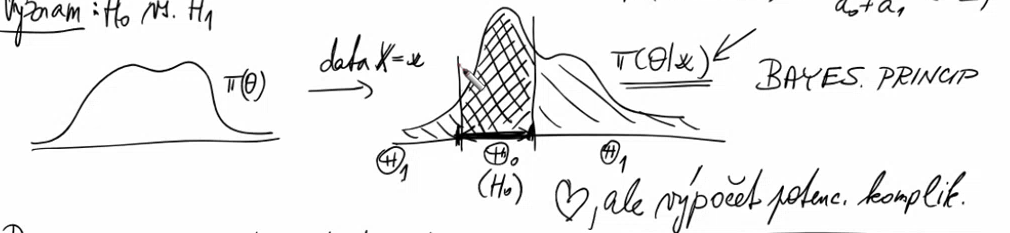
\includegraphics[width=0.7\linewidth]{pictures/last0}
			\caption{popis}
			\label{fig:last0}
		\end{figure}
		
		
		$$ \delta^\pi(\textbf{x})=\argmin_\delta \rho=\begin{cases}
		1&\text{pokud }a_1\PP^\pi(\t\in\Theta_1|\textbf{x})<a_0\PP^\pi(\t\in\Theta_0|\textbf{x}),\\
		0&\text{pokud }a_1\big(1-\PP^\pi(\t\in\Theta_0|\textbf{x})\big)<a_0\PP^\pi(\t\in\Theta_0|\textbf{x}),\\
		\end{cases} $$
		kde $\PP^\pi(\t\in\Theta_0|\textbf{x})>\frac{a_1}{a_0+a_1}\Big(=\frac{1}{2}\Big)$.
	\end{proof}
\end{theorem}
\begin{remark}
	Bayes umožňuje symetrizovat rozhodovací úlohu ($a_0=a_1$) nebo penalizovat v závislosti na úloze, experimentu nebo "datech"...
	
	B.TH se vyhýbá nutnosti nastavit $\alpha\in(0,1)$, protože $\alpha$ ovlivňuje $\beta$ sílu testu.
\end{remark}
\begin{define}
	Definujeme \textbf{Bayesovský faktor} jako$$ B^\pi(\textbf{x})=\frac{\frac{\PP^\pi(\t\in\Theta_0|\textbf{x})}{\PP^\pi(\t\in\Theta_0)}}{\frac{\PP^\pi(\t\in\Theta_0)}{\PP^\pi(\t\in\Theta_1)}}.$$
\end{define}
\begin{remark}
	Mějme například $\Theta_0=\{\t_0\}$, $\Theta_1=\{\t_1\}$, \[
	\begin{split}
	\PP^\pi(\t\in\Theta_0)=\PP(\t=\t_0)\equal{ozn}\pi_0,&\quad \PP^\pi(\t\in\Theta_1)=\PP(\t=\t_1)\equal{ozn}\pi_1\\ \PP^\pi(\t=\t_0|\textbf{x})=\pi(\t_0|\textbf{x})=\frac{f_0\pi_0}{f_0\pi_0+f_1\pi_1}&\quad \PP^\pi(\t=\t_1|\textbf{x})=\pi(\t_1|\textbf{x})=\frac{f_1\pi_1}{f_0\pi_0+f_1\pi_1}.
	\end{split}
	\]Z toho pak 
	$ B^\pi(\textbf{x})=\frac{\frac{f_0\pi_0}{f_1\pi_1}}{\frac{\pi_0}{\pi_1}}=\frac{f_0}{f_1}=\frac{L_0}{L_1}$ LR.
\end{remark}

Označme $\rho_0=\PP^\pi(\t\in\Theta_0)$, $\rho_1=\PP^\pi(\t\in\Theta_1)=1-\rho_0$. $H_0$ přijímáme, pokud $$a_1 \PP^\pi(\t\in\Theta_1|\textbf{x})<a_0\PP^\pi(\t\in\Theta_0|\textbf{x}),~(\delta(\textbf{x})=1),$$ 
kde 
$$ \PP^\pi(\t\in\Theta_1|\textbf{x})=\frac{a_1/a_0}{\rho_0/\rho_1}<\underbrace{\frac{\frac{\PP^\pi(\t\in\Theta_0|\textbf{x})}{\PP^\pi(\t\in\Theta_1|\textbf{x})}}{\frac{\rho_0}{\rho_1}}}_{B^\pi(\textbf{x})}.$$
\begin{remark}
	Sekvenční BTH: Máme $\rho_0,\rho_1$ a data $\textbf{x}$. Z toho pak $\pi(\t|\textbf{x})$, rozhodujeme mezi $H_0,H_1$, takže dostaneme $\tilde{\pi}(\t)=\pi(\t|\textbf{x})$ a data $\tilde{\textbf{x}}\sim \tilde{f}$. Potom $\tilde{\pi}(\t|\tilde{\textbf{x}}\textbf{x})$ a rozhodneme se mezi $H_0,H_1$. Dostaneme tak $\tilde{\tilde{\pi}}(\t)=\tilde{\pi}(\t|\tilde{\textbf{x}},\textbf{x})$ a pokračujeme dále analogicky.
\end{remark}


ASPEKT BTH:
Testujeme $\hypothesis{\t=\t_0}{\t\neq\t_0}$. Pokud $\t\sim\pi(\t)$ je spojitá hustota, pak 
$$ \rho_0=\PP^\pi(\t=\t_0)=0\quad\Rightarrow\quad \PP^\pi(\t=\t_0|\textbf{x})=\frac{f_0\pi_0}{c}=0,$$
případně analogicky pro $1$. Z toho zároveň vyplývá, že $\rho_0=\begin{cases}
0\\1
\end{cases}$ je absorbující stav. Dále víme, že $\pi(\t)$ je konstantní, tudíž nefreferujeme žádnou konkrétní hodnotu $\t\in\Theta$. 

\begin{example}
	Mějme $H_0$ hypotézu, že zítra bude pršet s pravděpodobností rovnu $0.7$ a $H_1$ jako $\neq 0.7$. Jak na to? Buď $$\hypothesis{\t\in(\t_0-\epsilon,\t_0+\epsilon)}{\t\notin(\t_0-\epsilon,\t_0+\epsilon)}$$
	nebo $\pi(\t)=\rho_0 \delta_{\t_0}+(1-\rho_0)\pi_1(\t)$, kde $\rho_0$ volíme větší, než $0$, případně menší, než $1$.
	
	\begin{figure}[h]
		\centering
		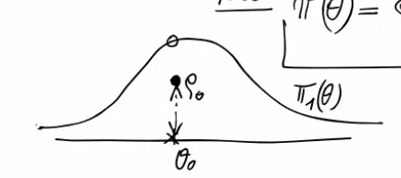
\includegraphics[width=0.5\linewidth]{pictures/last1}
		\caption{Tímto způsobem vnášíme do BTH dodatečnou apriorní informaci.}
		\label{fig:last1}
	\end{figure}
$$ \pi(\t_0|\textbf{x})=\PP^\pi(\t=\t_0|\textbf{x})=\frac{f_0\pi(\t_0)}{\int_\Theta \fex \pi\d\t}=\frac{f_0\rho_0}{f_0\rho_0+(1-\rho_0)\underbrace{\int_{\Theta_1}f\pi(\t)\d\t}_{m_1(\textbf{x})}}=\Big[1+\frac{1-\rho_0}{\rho_0}\frac{m_1(\textbf{x})}{f_0(\textbf{x})}\Big]^{-1}<\frac{a_1}{a_0+a_1},$$
tedy $B^\pi(\textbf{x}=\frac{f_0(\textbf{x})}{m_1(\textbf{x})})$.
\end{example}
\begin{example}
	Mějme $X\sim\NN(\mu,1)$ a $\hypothesis{\mu=0}{\mu\neq0}$, kde $\mu\in\R$. Víme, že $\rho_0=\frac{1}{2}$, $\rho_1=\frac{1}{2}$ (50:50). Potom
	\begin{enumerate}[a)]
		\item $$ \pi(\mu)=\frac{1}{2}\delta_0+\frac{1}{2}\pi(\t)=1\text{ na }\mu\neq0\quad(\text{nevlastní apriorní hustota}).$$
		potom $$ \pi(\mu=0|\textbf{x})=\frac{1}{1+\sqrt{2\pi} \e{x^2/2}}\stackrel{\forall x\in\R}{\leq}\frac{1}{1+\sqrt{2\pi}}=0.285\quad \text{vždy zamítáme }H_0!$$
		\item $\pi_1(\mu)=\NN(m=0,\tau^2)$ (vlastní), $\rho=\frac{1}{2}$, $\pi(\mu=0|\textbf{x})=[]^{-1}\stackrel{\tau\to+\infty}{\longrightarrow}1.$
		\begin{figure}[h]
			\centering
			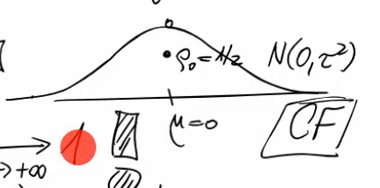
\includegraphics[width=0.5\linewidth]{pictures/last01}
			\caption{b)}
			\label{fig:last01}
		\end{figure}
		
	\end{enumerate}
$$ \begin{array}{c|c|c|c|c|c}
x & 0 & 0.68 & 1.28 & 1.96 & ... \\\hline
\substack{\pi(0|x)\\ \tau=1}& 0.586 & 0.557 & 0.484 & 0.351 & ... \\\hline
\substack{\pi(0|x)\\ \tau=10}& 0.768 & 0.729 & 0.612 & 0.366 & ...
\end{array}
 $$
\end{example}
\begin{figure}[h]
	\centering
	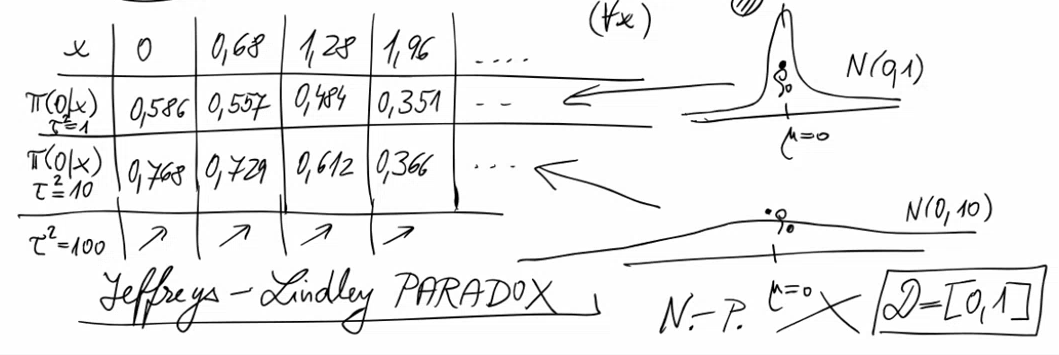
\includegraphics[width=0.8\linewidth]{pictures/last02}
	\caption{Jeffreys-Lindley Paradox}
	\label{fig:last02}
\end{figure}
